%% It is just an empty TeX file.
%% Write your code here.
%\documentclass{beamer}
%\setbeamertemplate{navigation symbols}{}

%\usepackage{beamerthemeshadow}

% added packages by JW:
%\usepackage{amsmath}
%\begin{document}
\section{Introduction}
\label{sec:introduction}




\begin{frame}\frametitle{Problem Statement}
\begin{itemize}
\item Solid state physics: electronic structure computation
\begin{itemize}
\item \(\rightarrow\) Fleur: electronic structure of crystals using DFT
\item Fleur simulation code developed and maintained by Institute of Advanced Simulation-1 at FZJ and is open source
\item huge amount of data
\item physics not accessible unless structured / analysed / visualized
\end{itemize}
\end{itemize}
%FLEUR is the simulation code developed by 
The goal of the project was to implement a complete data analysis pipeline for this application:
\begin{itemize}
\item preprocessing \(\rightarrow\) data exploration \(\rightarrow\) visualization
\end{itemize}
\end{frame}

\begin{frame}\frametitle{Motivation \& Requirements}
\begin{itemize}
\item to solve physicist's problems with the simulation data
\item process Fleur output files
\item modularization \& easy maintainability of code
\item fast computation time
\item frontend: no installation required, intuitive usage
\item high-quality export features
\end{itemize}
\end{frame}

\begin{frame}[plain]
\frametitle{Visualisation}
\begin{figure}
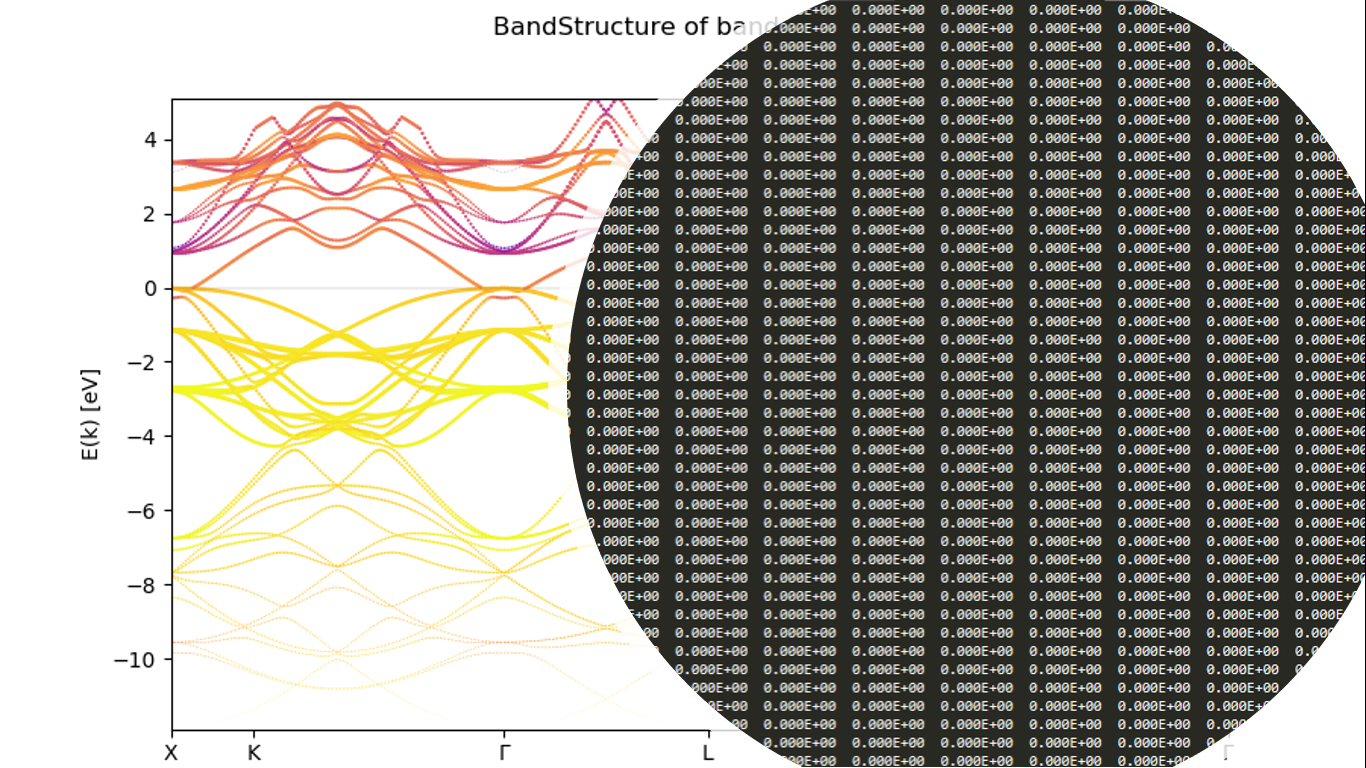
\includegraphics[scale=0.25]{fig/visual} 
\caption{Transformation}
\end{figure}
\end{frame}

\begin{frame}\frametitle{Steps}
\begin{itemize}
\item understanding physics and problem
\item preprocessing the data
\item exploring the data(implementation)
\item visualization \& GUI
\item results
\end{itemize}
\end{frame}



%\end{document}